%\newpage
\subsection{Оперативное планирование производства}
\label{bp:OperPlan}

Все заявки от покупателей  менеджеры отдела продаж регистрируют в системе 1C:УПП (рис. \ref{pic:2.1 Заказы в УПП_0001}). 

%Менеджер выгружает в отдел планирования в системе СБИС заявки покупателей. 
Специалист по планированию производства (ПП) производит перенос заказов из 1C:УПП в документ MS Excel "AVA заказы" (рис. \ref{pic:2.1 Заказы в файле эксель АВА_0001}). Специалист ПП производит перенос заказов несколько раз в течение рабочего дня. Регламент приема заказов отсутствует. Задача --- набрать объем заказов для обеспечения загрузки производства. Специалист ПП ориентируется на желаемую дату производства, которую указал менеджер. Возможно срочное добавление заказов. Заказы, которые последними перенесены из системы  1С: УПП, вставляются в конец списка. По каждому заказу  ориентируясь на ТК и свой опыт  специалист ПП указывает маршрут для производства. Специалист ПП переносит заказы на вкладку "Каталог заказов". По каждому заказу в ручную переносятся данные по размерам заготовок, марке и профилю (рис. \ref{pic:2.4 каталог заказов_0001}). 
На предприятии организовано планирование от линий переработки. 

\textbf{Планирование линий переработки}

Для  планирования ручных и автоматических линий переработки специалист ПП переходит в файл MS Excel "Драм" (рис. \ref{pic:2.6 Задание на ручной станок в Драм_0001}). Задания на ручные линии переработки указывается без расчета времени на выработку заказа. На автоматические линии расчет времени производится исходя из плановой производительности  без учета сложности изготовления (рис. \ref{pic:2.6 задание на линию в Драм_0001}). Плановая производительность устанавливается генеральным директором (рис. \ref{pic:4 План выработки в шт}). Время переналадки и технологические перерывы не учитываются. Время начала работы каждой линии переработки указывается. 
Специалист ПП печатает задания на сетевой принтер, установленный на производстве у начальника смены, в 15-30 на вечернюю смену и следующую смену.

Каждое утро рабочего дня специалист ПП формирует в системе 1С:УПП отчет по выработке продукции (рис. \ref{pic:0 Отчет выпуск продукции и услуг_0001}) и сравнивает данные с файлом MS Excel "Драм". В файле  "Драм" в ручную переносятся данные о выработке заказов. Если отклонение от выпуска по заказу превышает 5 процентов, то специалист ПП совместно с менеджером принимает решение --- считать заказ выработанным или нет. Если отклонение менее 5 процентов, то специалист ПП самостоятельно удаляет заказ из очереди. 

\textbf{Планирование выпуска на гофроагрегате}

На каждый заказ производства менеджер создает новую характеристику номенклатуры в системе 1С:УПП копированием ТК. Таким образом планирование выполняется не по заказам, а по коду характеристики в системе 1С:УПП.


Планирование и создание заданий  на выпуск продукции и заготовок на гофроагрегате производится в файле MS Excel ''Драм'' (рис. \ref{pic:0 Крой в эксель_0001}). Основные форматы, используемые при крое: 2000 мм, 2100 мм, 2500 мм. Дополнительно может быть использован формат 2450 мм. Выпускаемые профили гофры: В,С,Е,ВС, ВЕ. Максимальное количество полос для кроя --- 6 полос. Планирование гофроагрегата ведется от загруженности линий переработки с учетом типов выпускаемых изделий. Планирование осуществляется только на смену с 8-00 до 20-00. План выпуска на смену установлен 138600 м2. Допустимая кромка отхода по полотну составляет 3\%. Количество раскроев на смену в среднем составляет более 20.

Из документа MS Excel "АВА заказ" специалист ПП вручную переносит размеры заготовок по каждому заказу. Исходя из своего опыта специалист ПП собирает вручную "блоки" по форматам, профилям и маркам.  Специалист ПП вручную производит поиск подкроя для каждого заказа, ориентируясь на значение кромки. Рилевки проверяются также вручную. Часто возникают проблемы с поиском подкроя к заказам на профилях: ВС, ВЕ, Е и высоких марках из-за небольшого количества заказов. Сырье для выработки заказов проставляется вручную с учетом утвержденных композиций (рис. \ref{pic:0 Композиции сырья_0001}).
Специалист ПП для качественного кроя гофрополотна может создавать раскрой без заказа. Поэтому кроится все с минимальной обрезью. 
Таким образом на ГА выполняется перевыпуск, который не виден по отчетам.

После создания раскроев специалист ПП формирует задание на выпуск заготовок и готовой продукции на гофроагрегате. (рис. \ref{pic:2.8.3 задание от плановика на производство_0001.jpg}). Задание отправляется начальникам смен в электронной почте и "WhatsApp". 
Начальники смен  при получении плана работы могут самостоятельно распределяет задания по линиям исходя из загруженности линий, возможности производства. 

Специалист ПП контролирует остатки по сырью. Если сырья не хватает, специалист ПП сообщает в отдел закупок, что по конкретным позициям сырья образовался дефицит.


\clearpage
%\clearpage

 
%Инженер в системе СБИС выгружает заявки в систему планирования PMASC. 
%Система СБИС выгружает заявку полностью. В заявке может быть несколько строк (заказов). В систему PMASC заявка загружается с номером СБИС, номер заказа указывается как номер заявки СБИС + номер строки в заявке.
%Менеджеры могут прикрепить в СБИС файлы с макетами и оснасткой.


%Система PMASC позволяет для загруженных заявок сформировать оптимальные схемы раскроя гофрополотна по заданным параметрам.
%В системе по умолчанию инженер БППП указывает дату между заказами в раскрое 1 день. Это позволяет кроить заказы, которые менеджеры поставили в один желаемый день производства. Крой выполняется по марке. Оперативные остатки по сырью (бумага и картон) инженер БППП получает из системы СБИС %(рис. \ref{pic:d6}).   

%В ходе обследования выявлены нормативные марки и состав композиций  %(рис. \ref{pic:d7}).  
%ормативы по композициям устаревшие и требуют обновления.
%алее инженер БППП в системе PMASC выполняет автоматический поиск раскроев, редактирует список раскроев и подбирает композиции сырья вручную. 
%охраненные и принятые в работу раскрои инженер БППП экспортирует из системы
 %PMASC в систему СБИС через файлы обмена формата xml. 
%Загруженные раскрои в системе СБИС находятся в журнале раскроев %(рис. \ref{pic:d7}). 
%В системе СБИС есть возможность смотреть план, но менеджеры не используют эту возможность, потому как нужно переключать модуль в виду отсутствия возможности работы одновременно в разных режимах.

%Инженер БППП печатает крой %(рис. \ref{pic:dd10}) в количестве 9 экземпляров.
%Задание (крой) передается в коммерческий отдел для планирования производства.
%Менеджеры коммерческого отдела выбирают в заданиях в крой те заказы, которые нужно брать в работу с учетом желаемой даты производства.
%Раскрои с датами заместитель директора по производству возвращает от менеджеров в БППП.
%Заместитель директора по производству указывает композицию сырья в раскроях по плану и передает задание на гофроагрегат в цех, через мастера производства.




%Каждый день инженер БППП создает отчет по заготовкам, выпущенным с гофроагрегата %(рис. \ref{pic:d14}) вручную. 
%Инженер БППП в системе PMASC создает план на переработку вручную: план на ящики, отдельно план на сложную высечку, отдельно план на изготовление решетки и прокладки.
%Инженер БППП печатает задание на линию из системы PMASC %(рис. \ref{pic:d15}) и передает мастеру производства. 

%Задания передаются операторам линий переработки. 

\begin{figure}
\begin{center}
  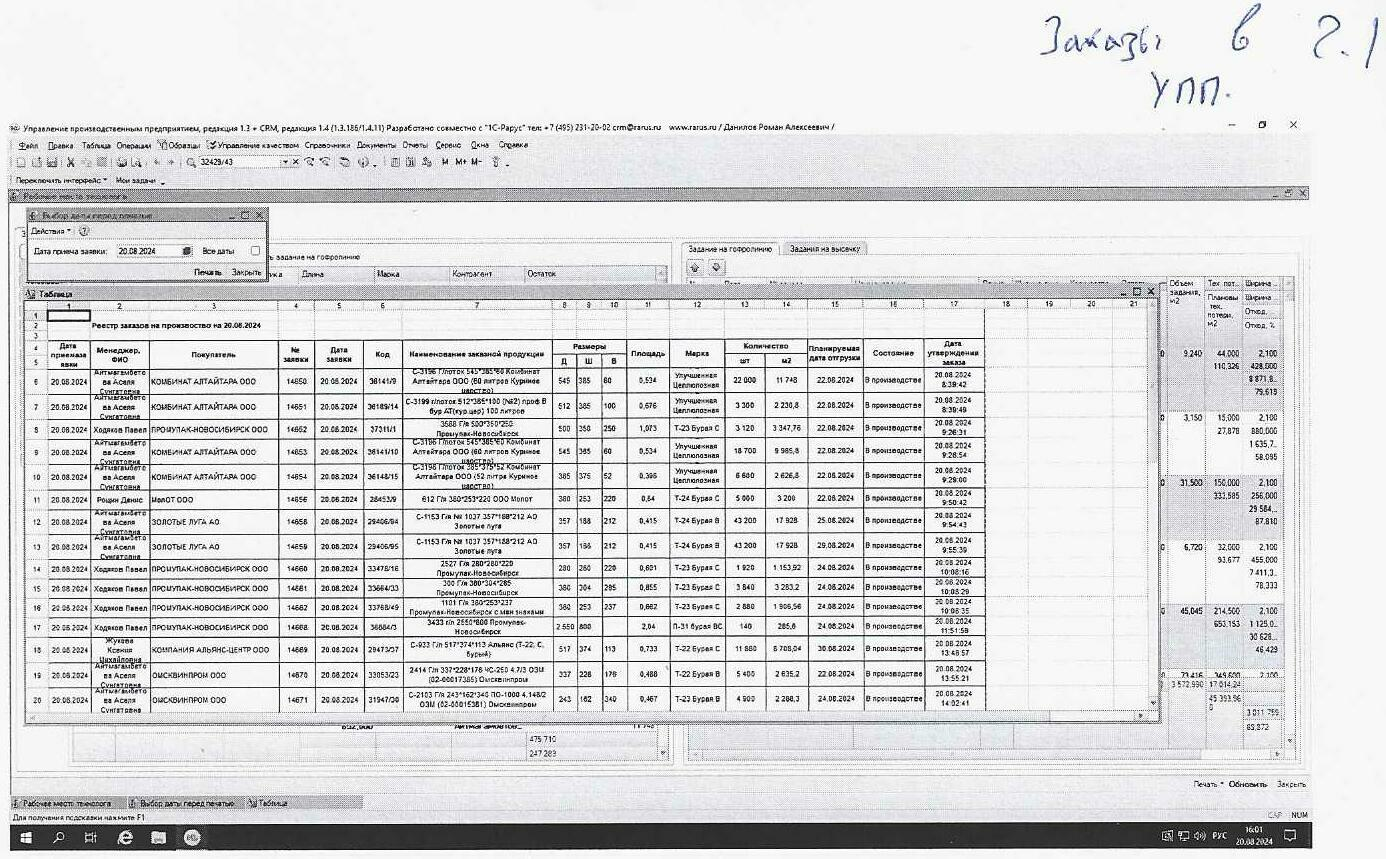
\includegraphics[height=0.94\textheight, width=0.94\textwidth, keepaspectratio]{Pics 1/2.1 Заказы в УПП_0001.jpg }
\end{center}
  \caption{Заказы в системе 1С:УПП}
  \label{pic:2.1 Заказы в УПП_0001}
\end{figure}

\begin{figure}
\begin{center}
  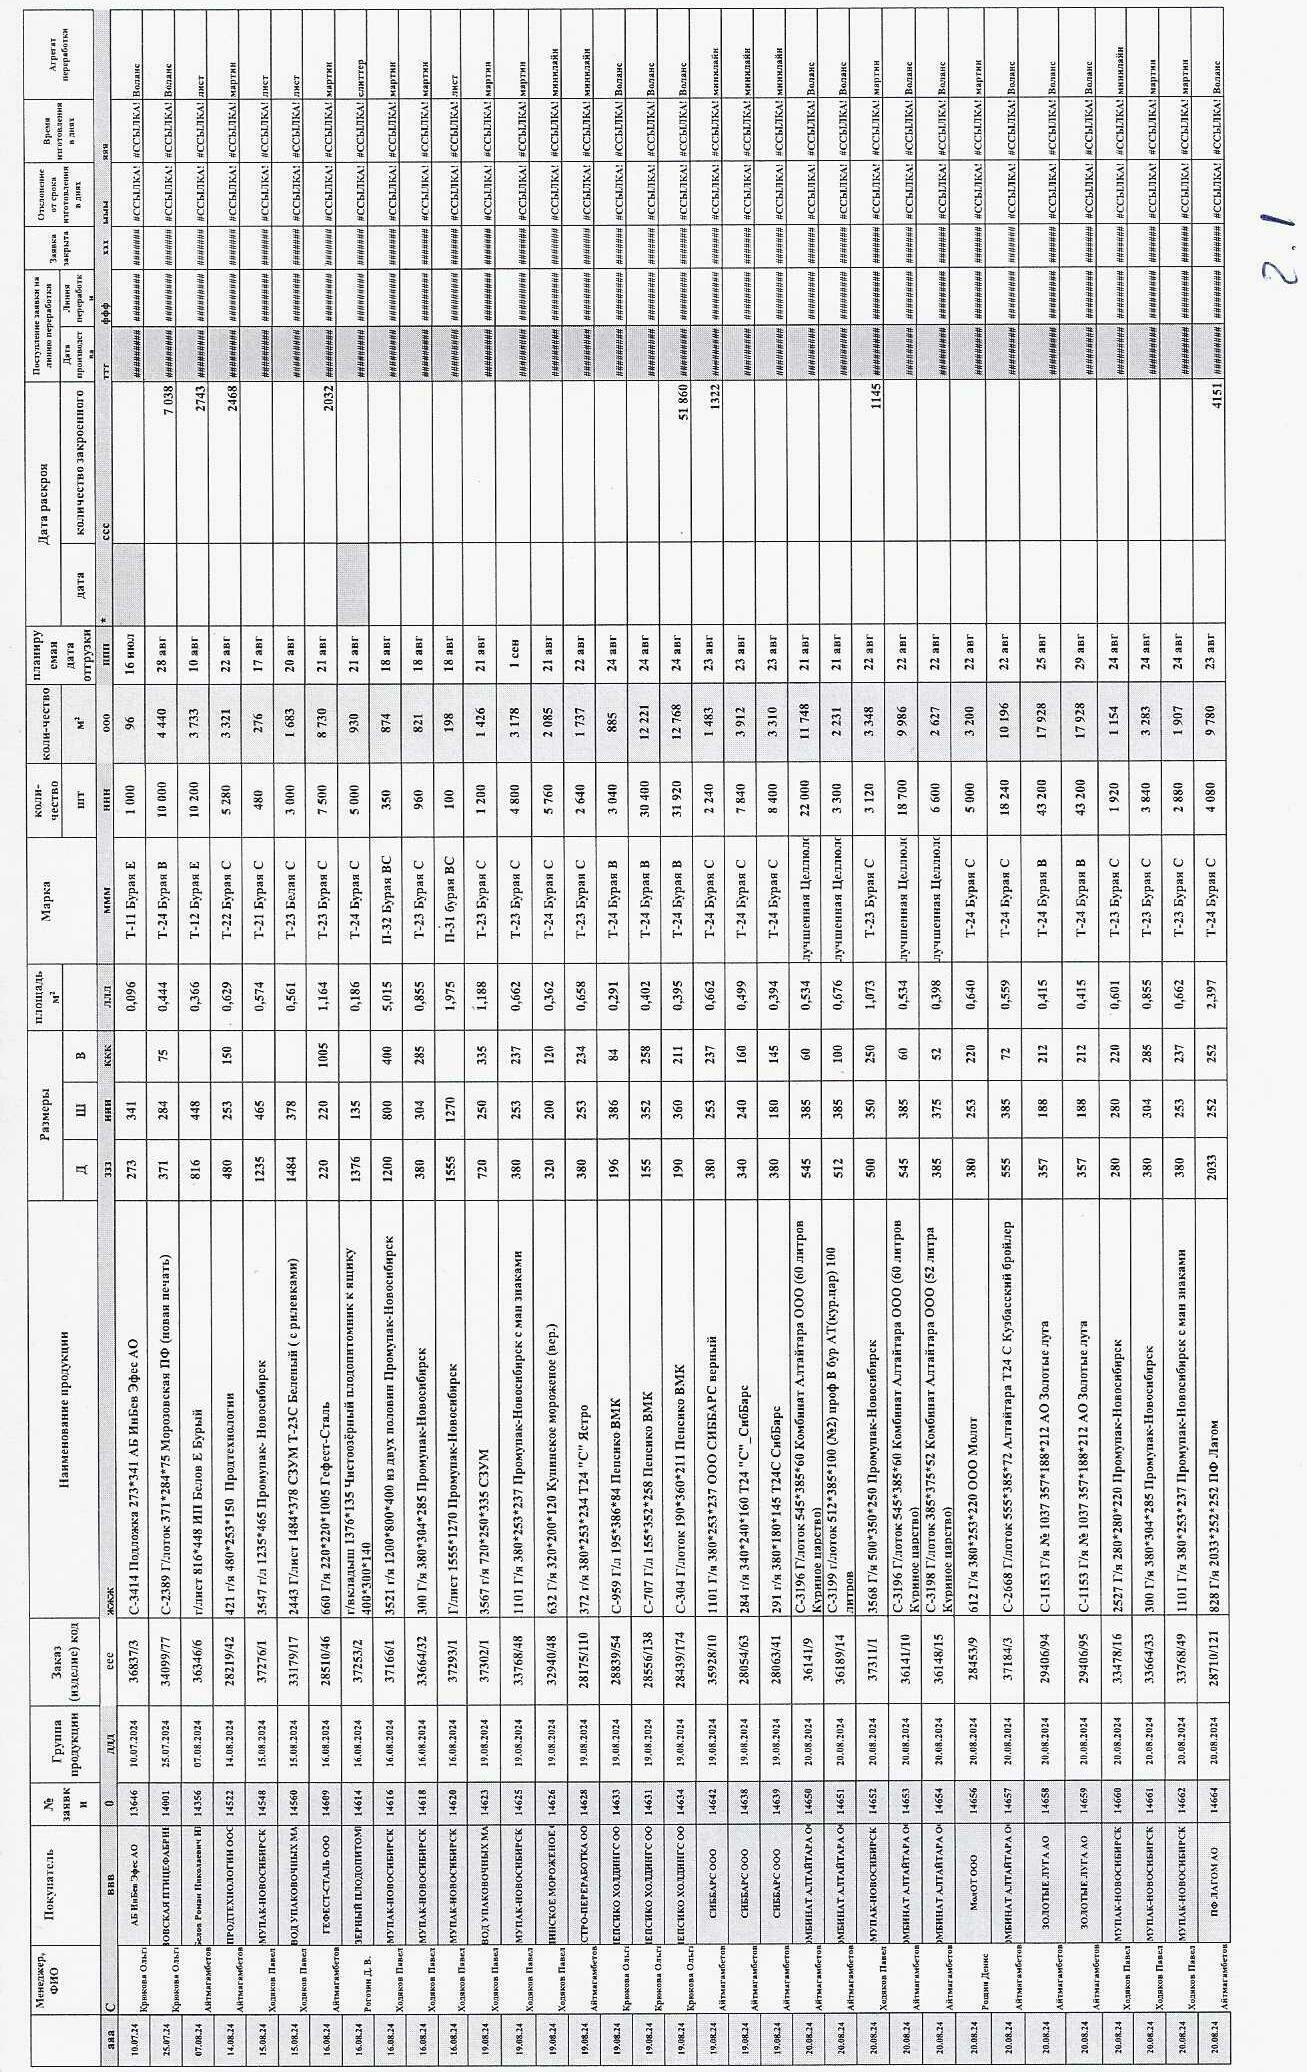
\includegraphics[height=0.94\textheight, width=0.94\textwidth, keepaspectratio]{Pics 1/2.1 Заказы в файле эксель АВА_0001.jpg}
\end{center}
  \caption{Заказы в MS Excel}
  \label{pic:2.1 Заказы в файле эксель АВА_0001}
\end{figure}

\begin{figure}
\begin{center}
  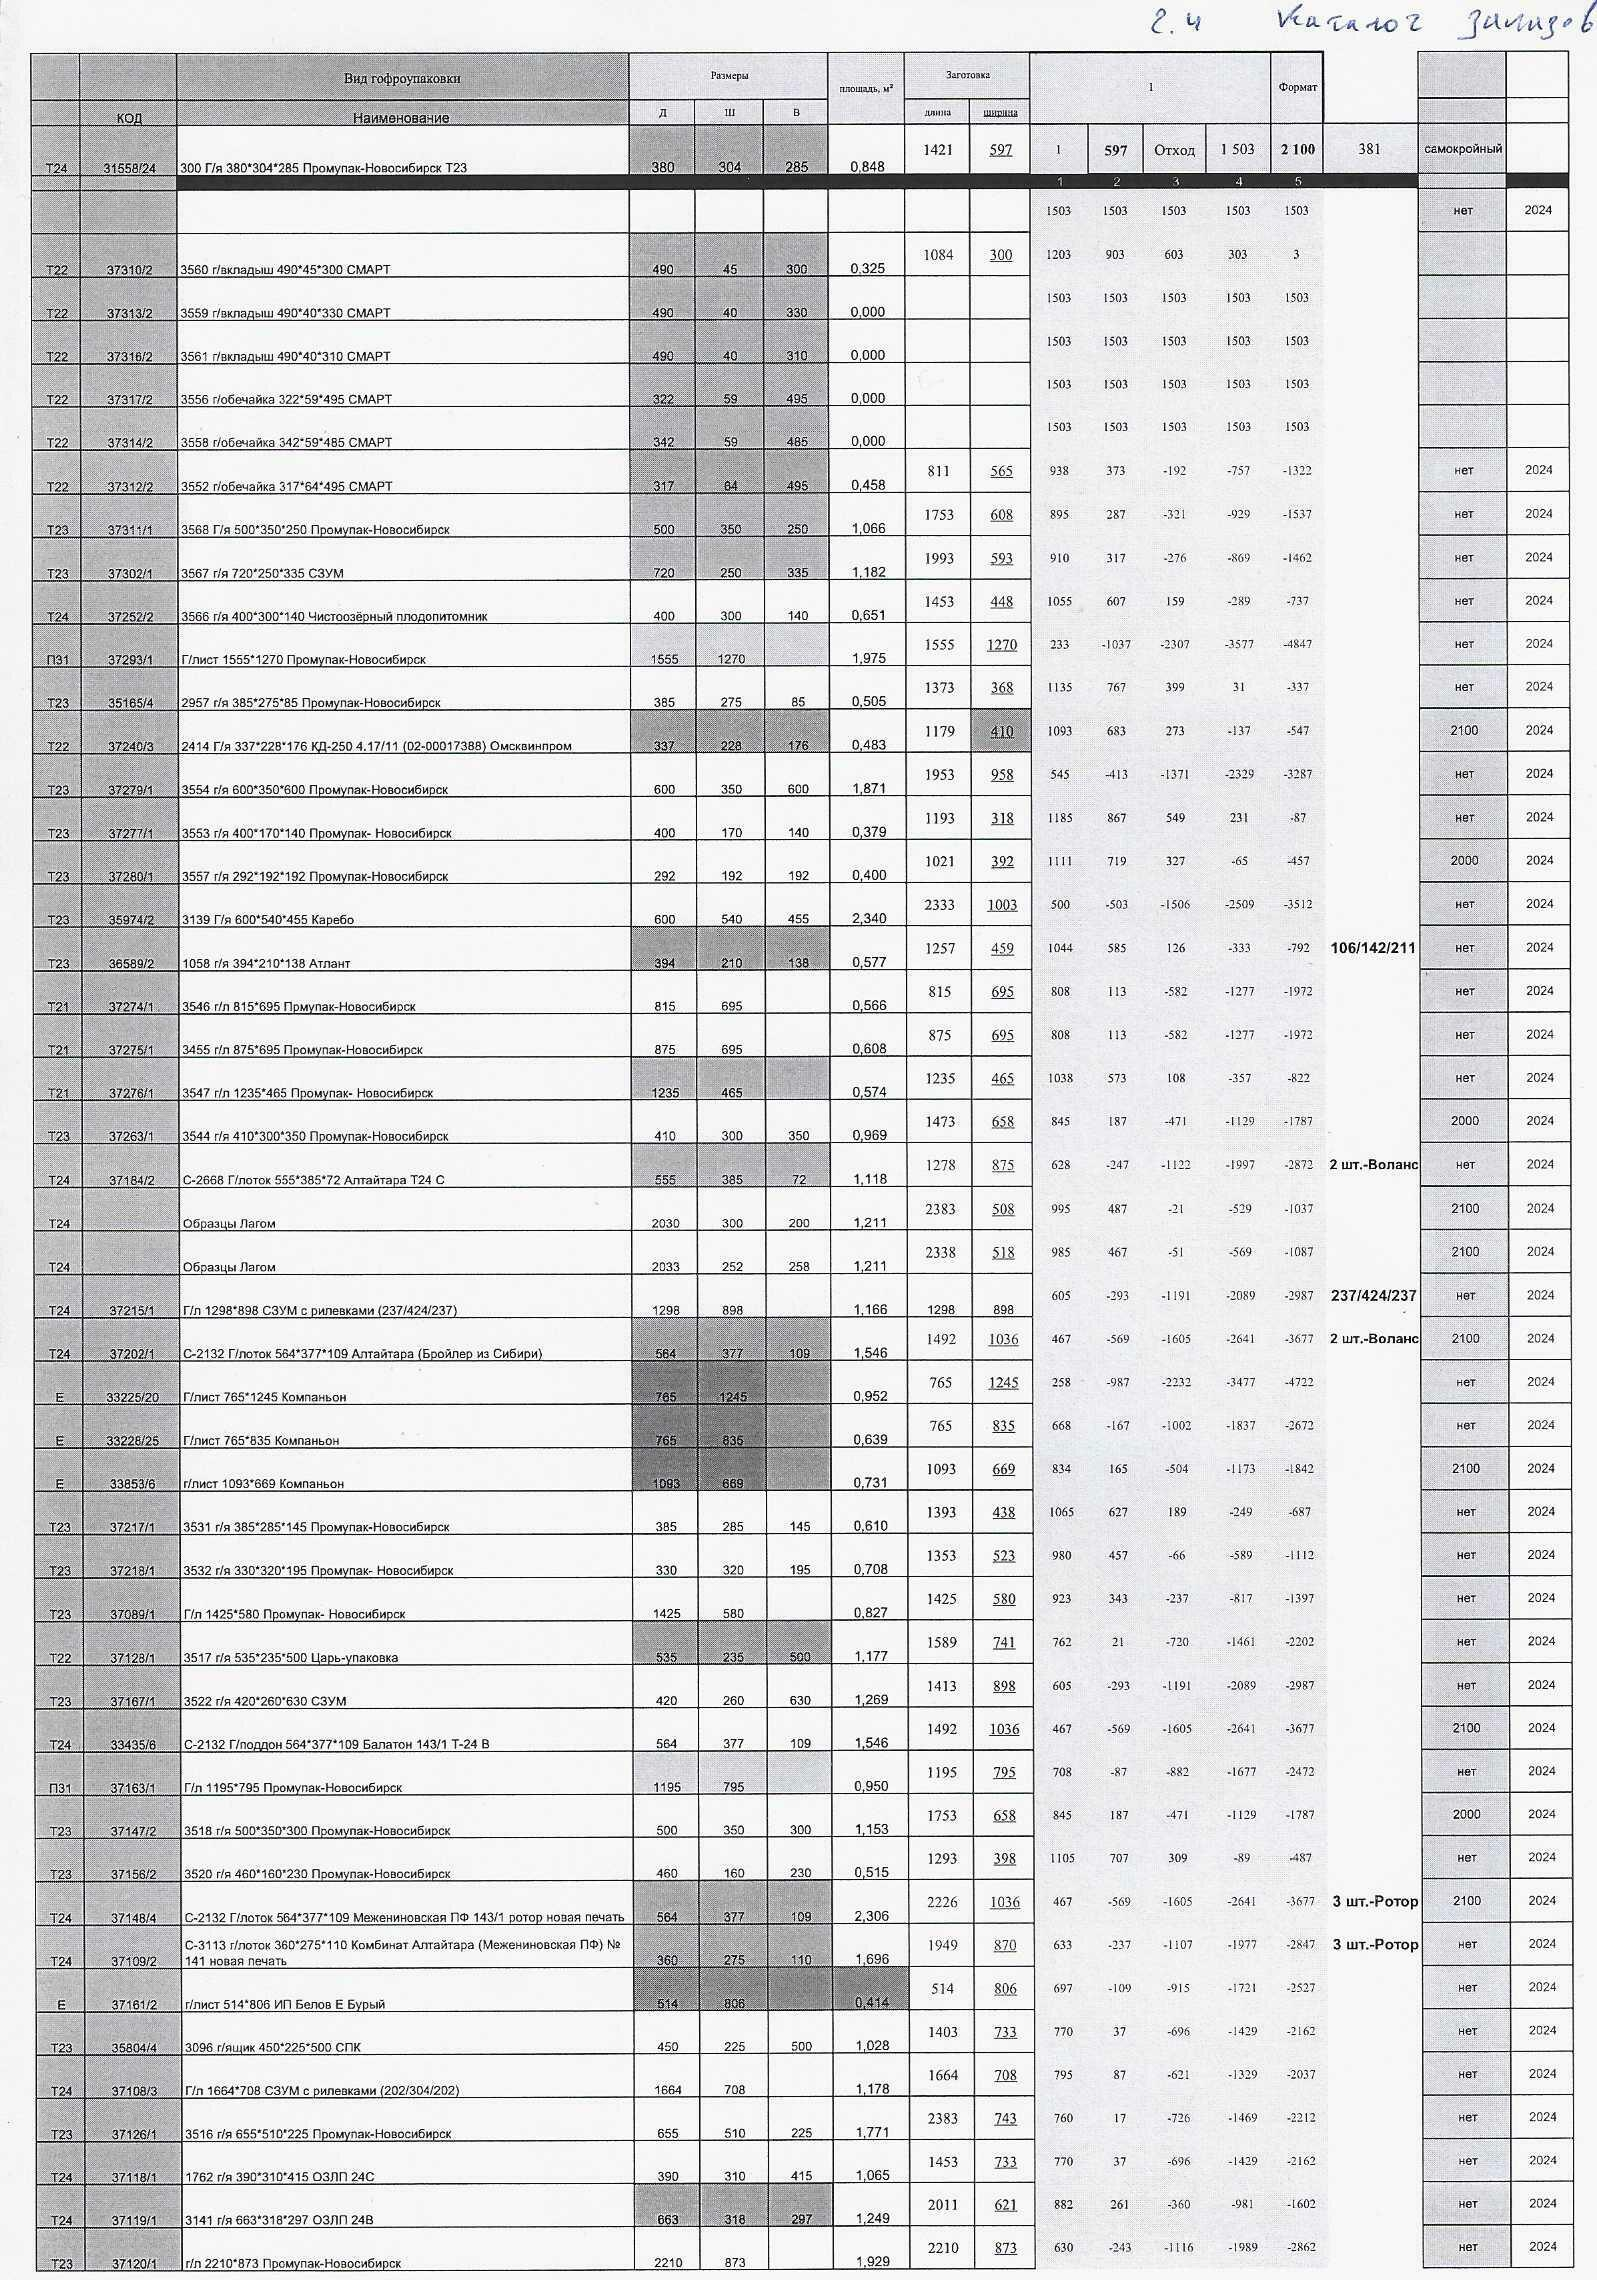
\includegraphics[height=0.94\textheight, width=0.94\textwidth, keepaspectratio]{Pics 1/2.4 каталог заказов_0001.jpg}
\end{center}
  \caption{Каталог заказов в MS Excel}
  \label{pic:2.4 каталог заказов_0001}
\end{figure}

\begin{figure}
\begin{center}
  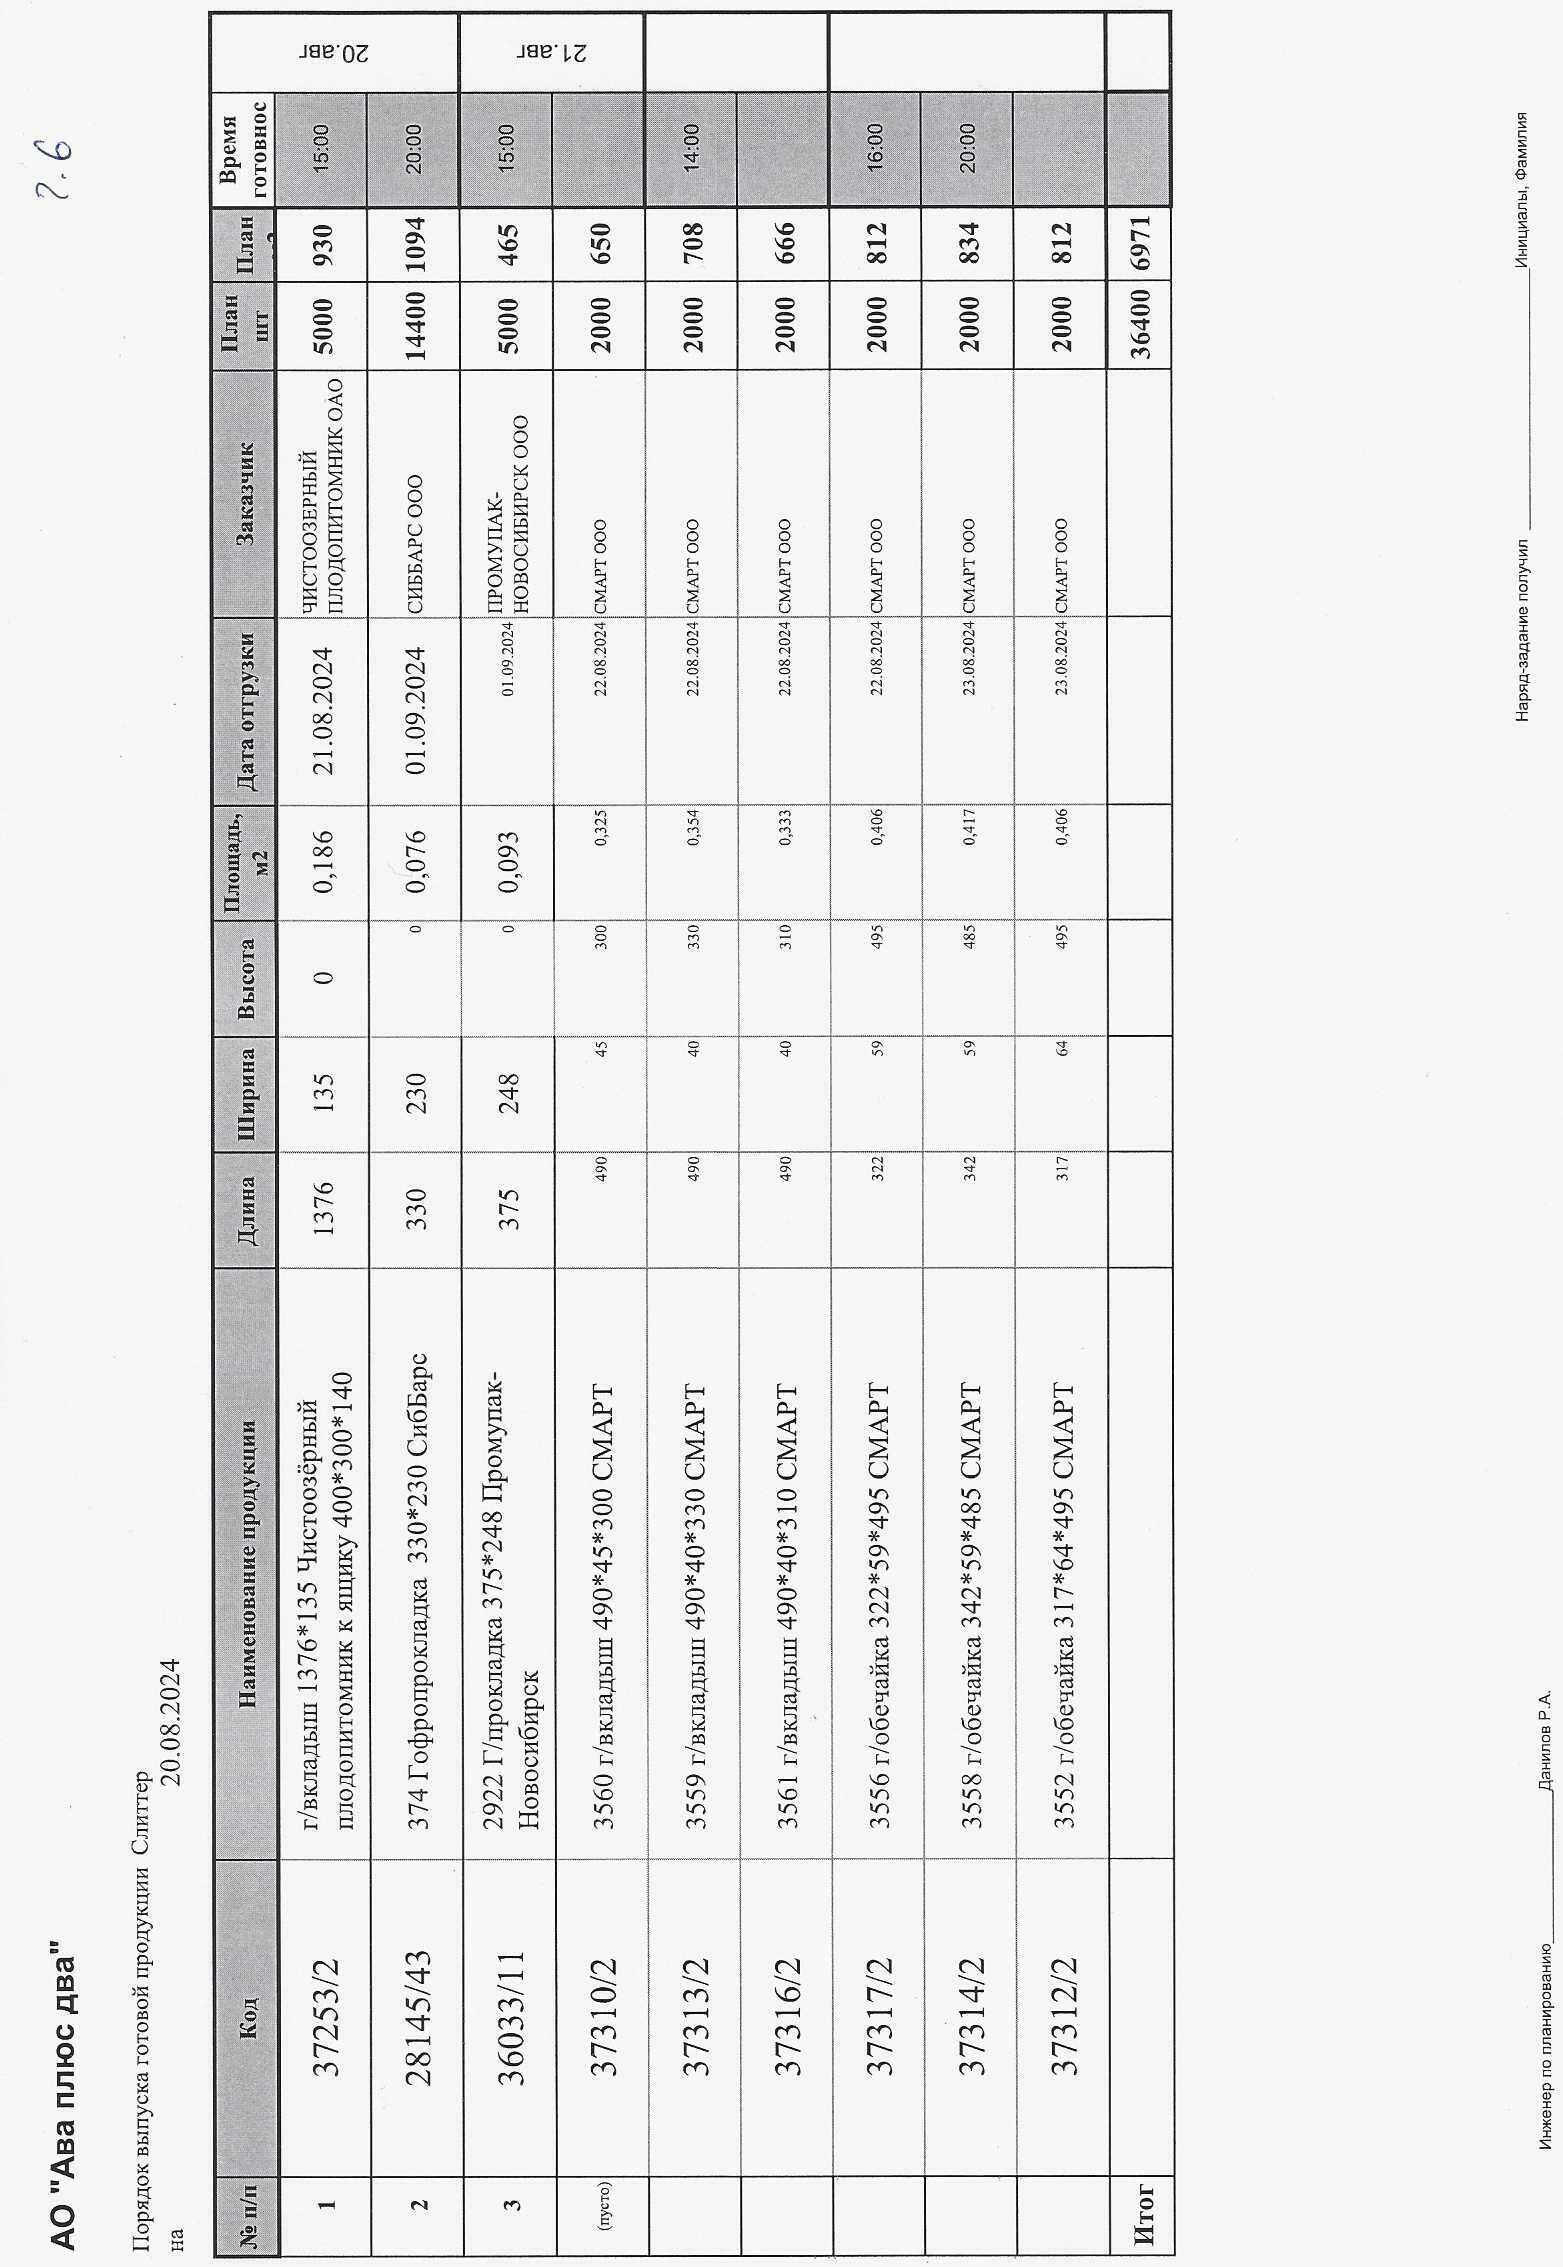
\includegraphics[height=0.94\textheight, width=0.94\textwidth, keepaspectratio]{Pics 1/2.6 Задание на ручной станок в Драм_0001.jpg}
\end{center}
  \caption{Задания на ручной станок}
  \label{pic:2.6 Задание на ручной станок в Драм_0001}
\end{figure}

\begin{figure}
\begin{center}
  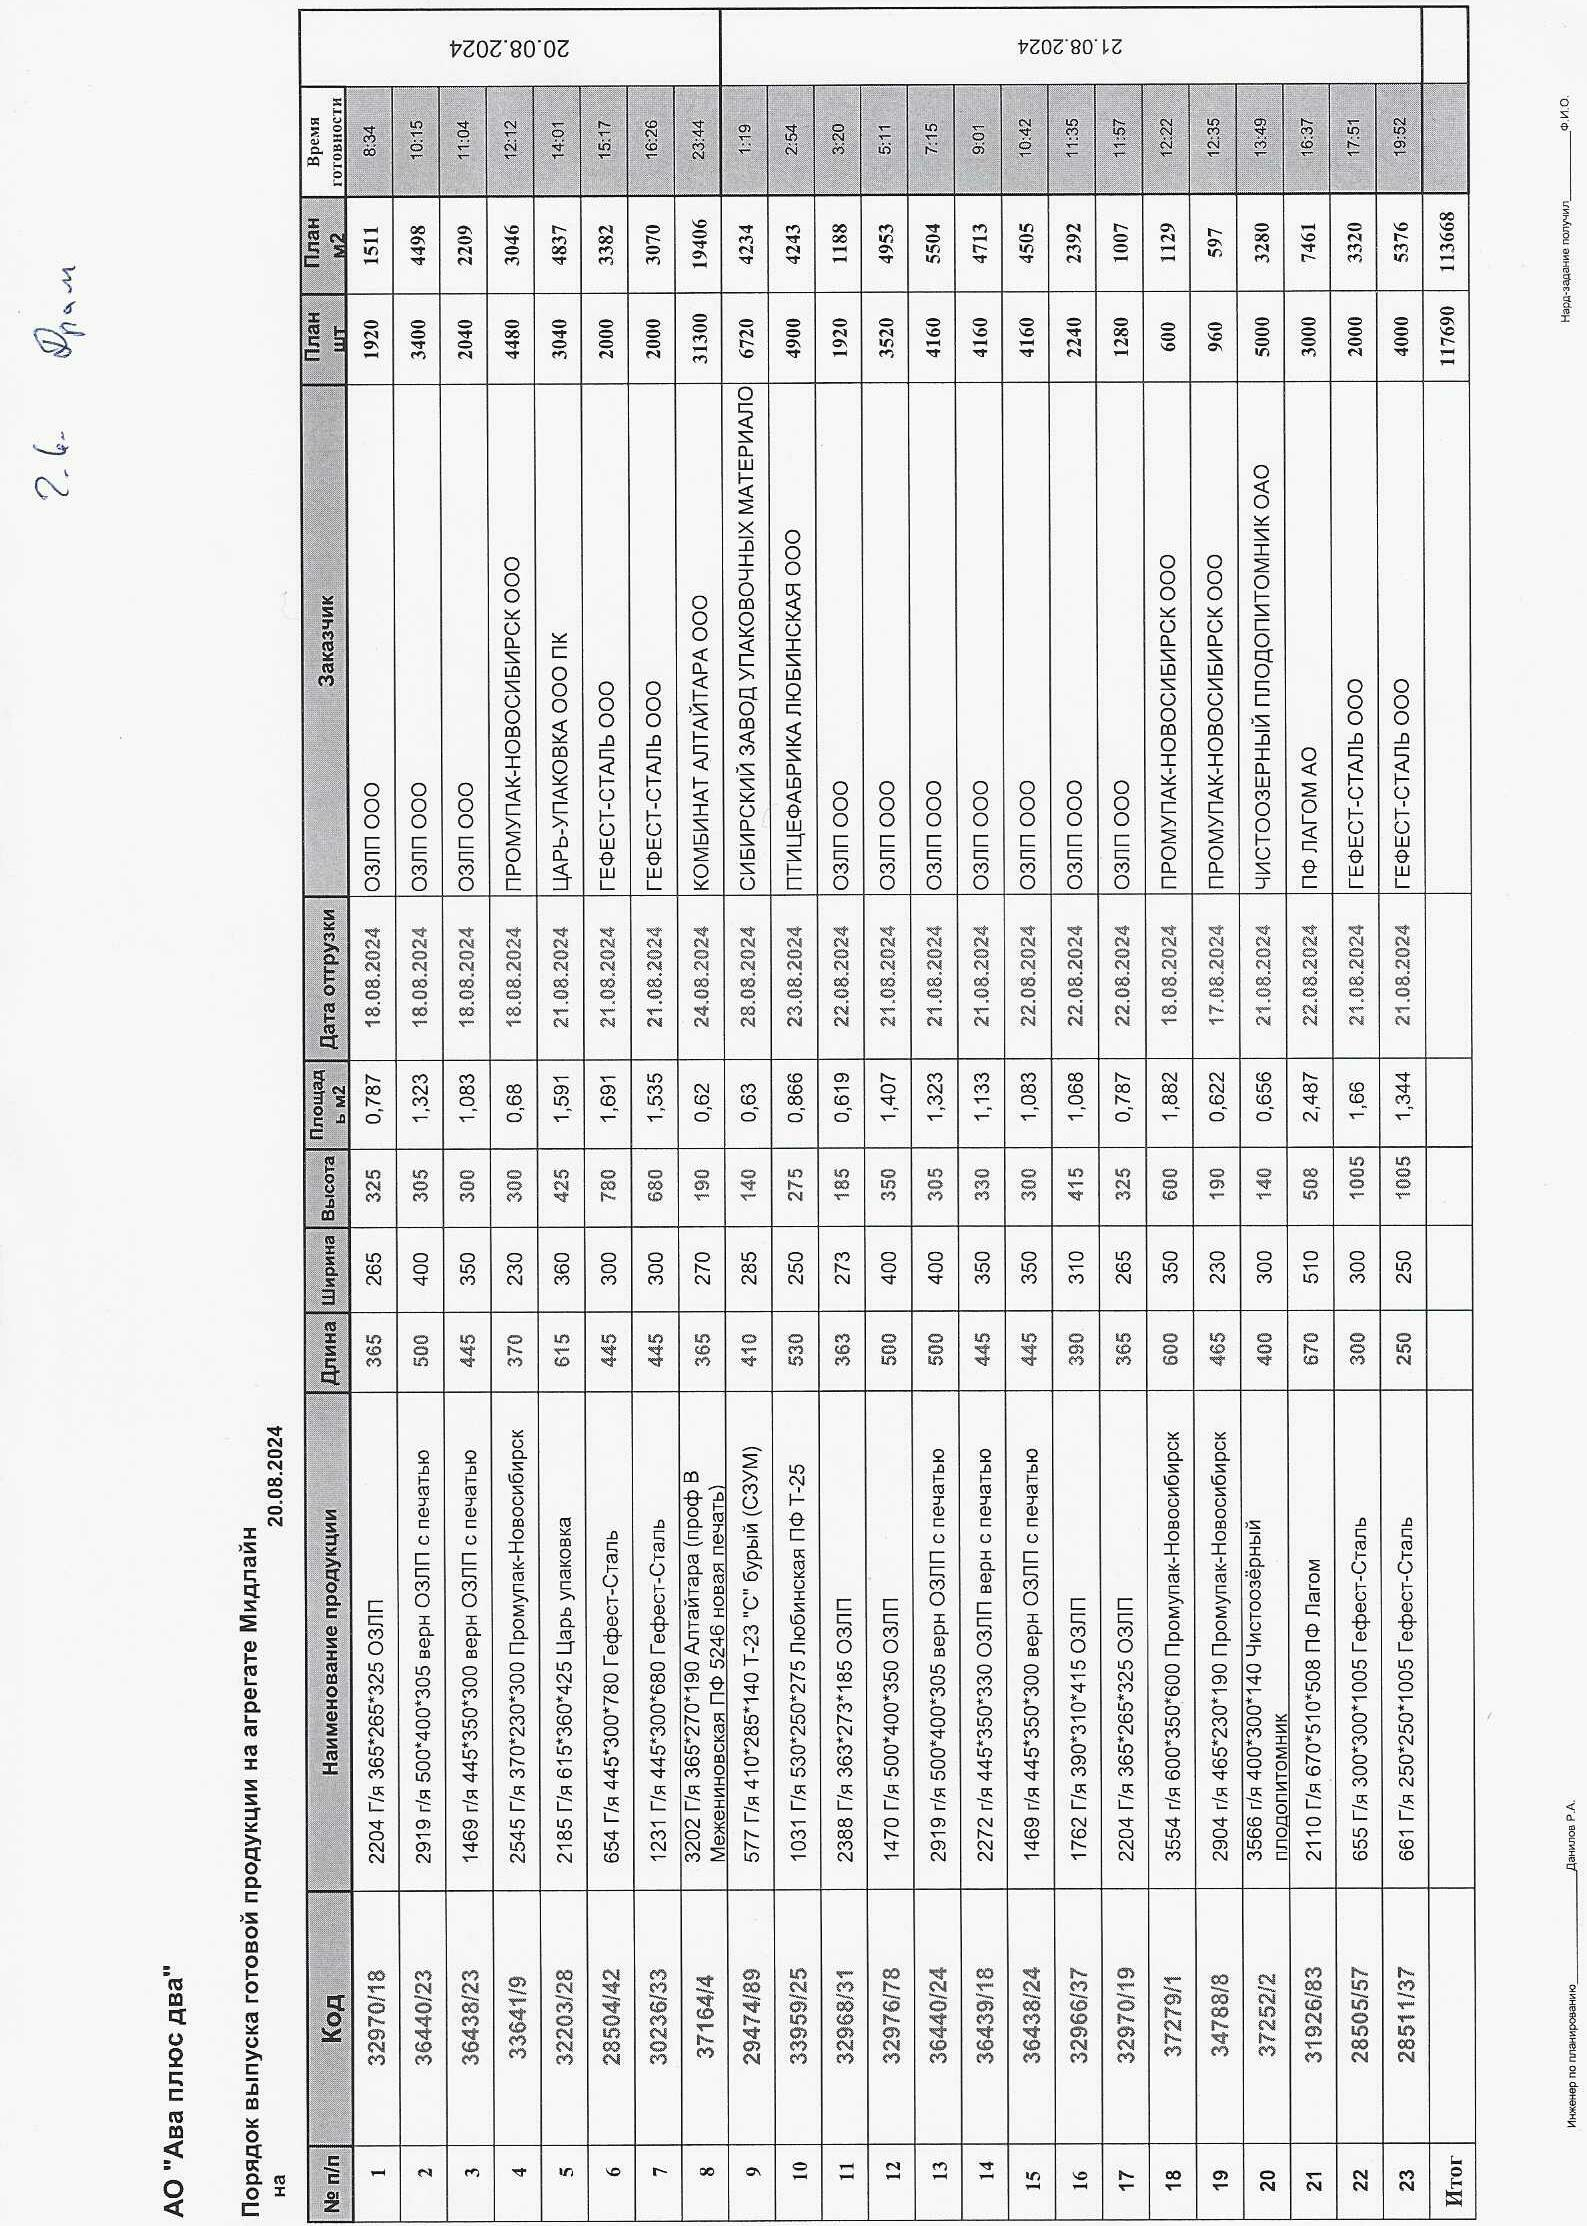
\includegraphics[height=0.94\textheight, width=0.94\textwidth, keepaspectratio]{Pics 1/2.6 задание на линию в Драм_0001.jpg}
\end{center}
  \caption{Задание на автоматическую линию}
  \label{pic:2.6 задание на линию в Драм_0001}
\end{figure}

\begin{figure}
\begin{center}
  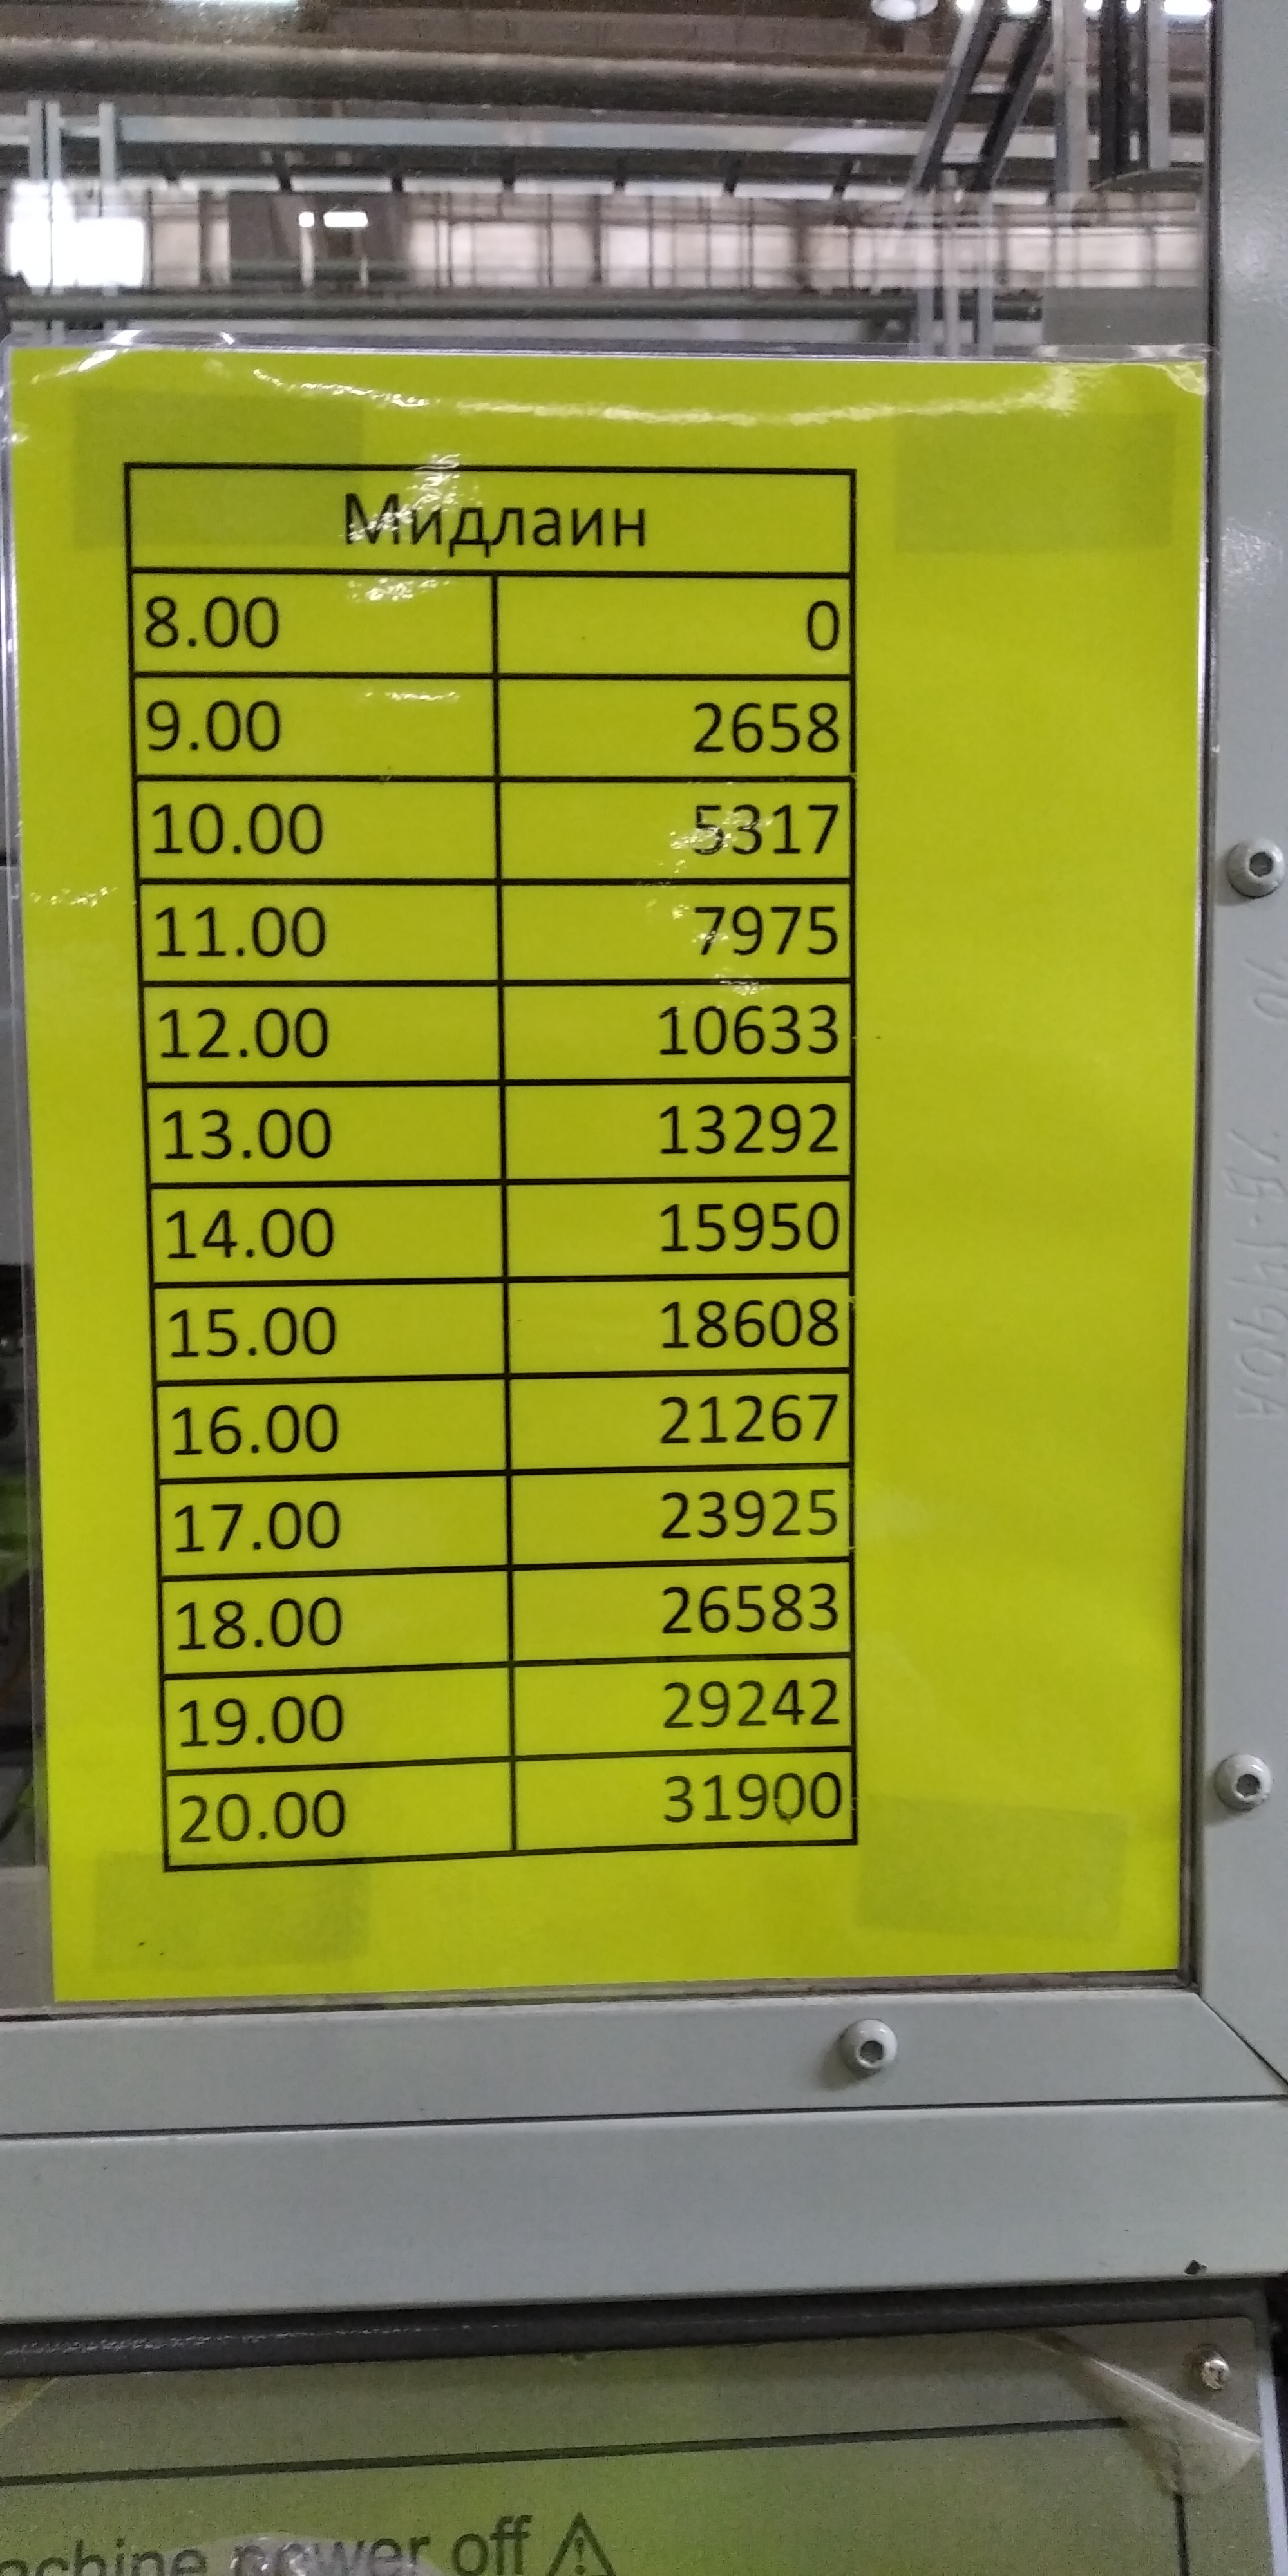
\includegraphics[height=0.94\textheight, width=0.94\textwidth, keepaspectratio]{Pics 1/4 План выработки в шт..jpg}
\end{center}
  \caption{Плановая выработка}
  \label{pic:4 План выработки в шт}
\end{figure}

 \begin{figure}
\begin{center}
  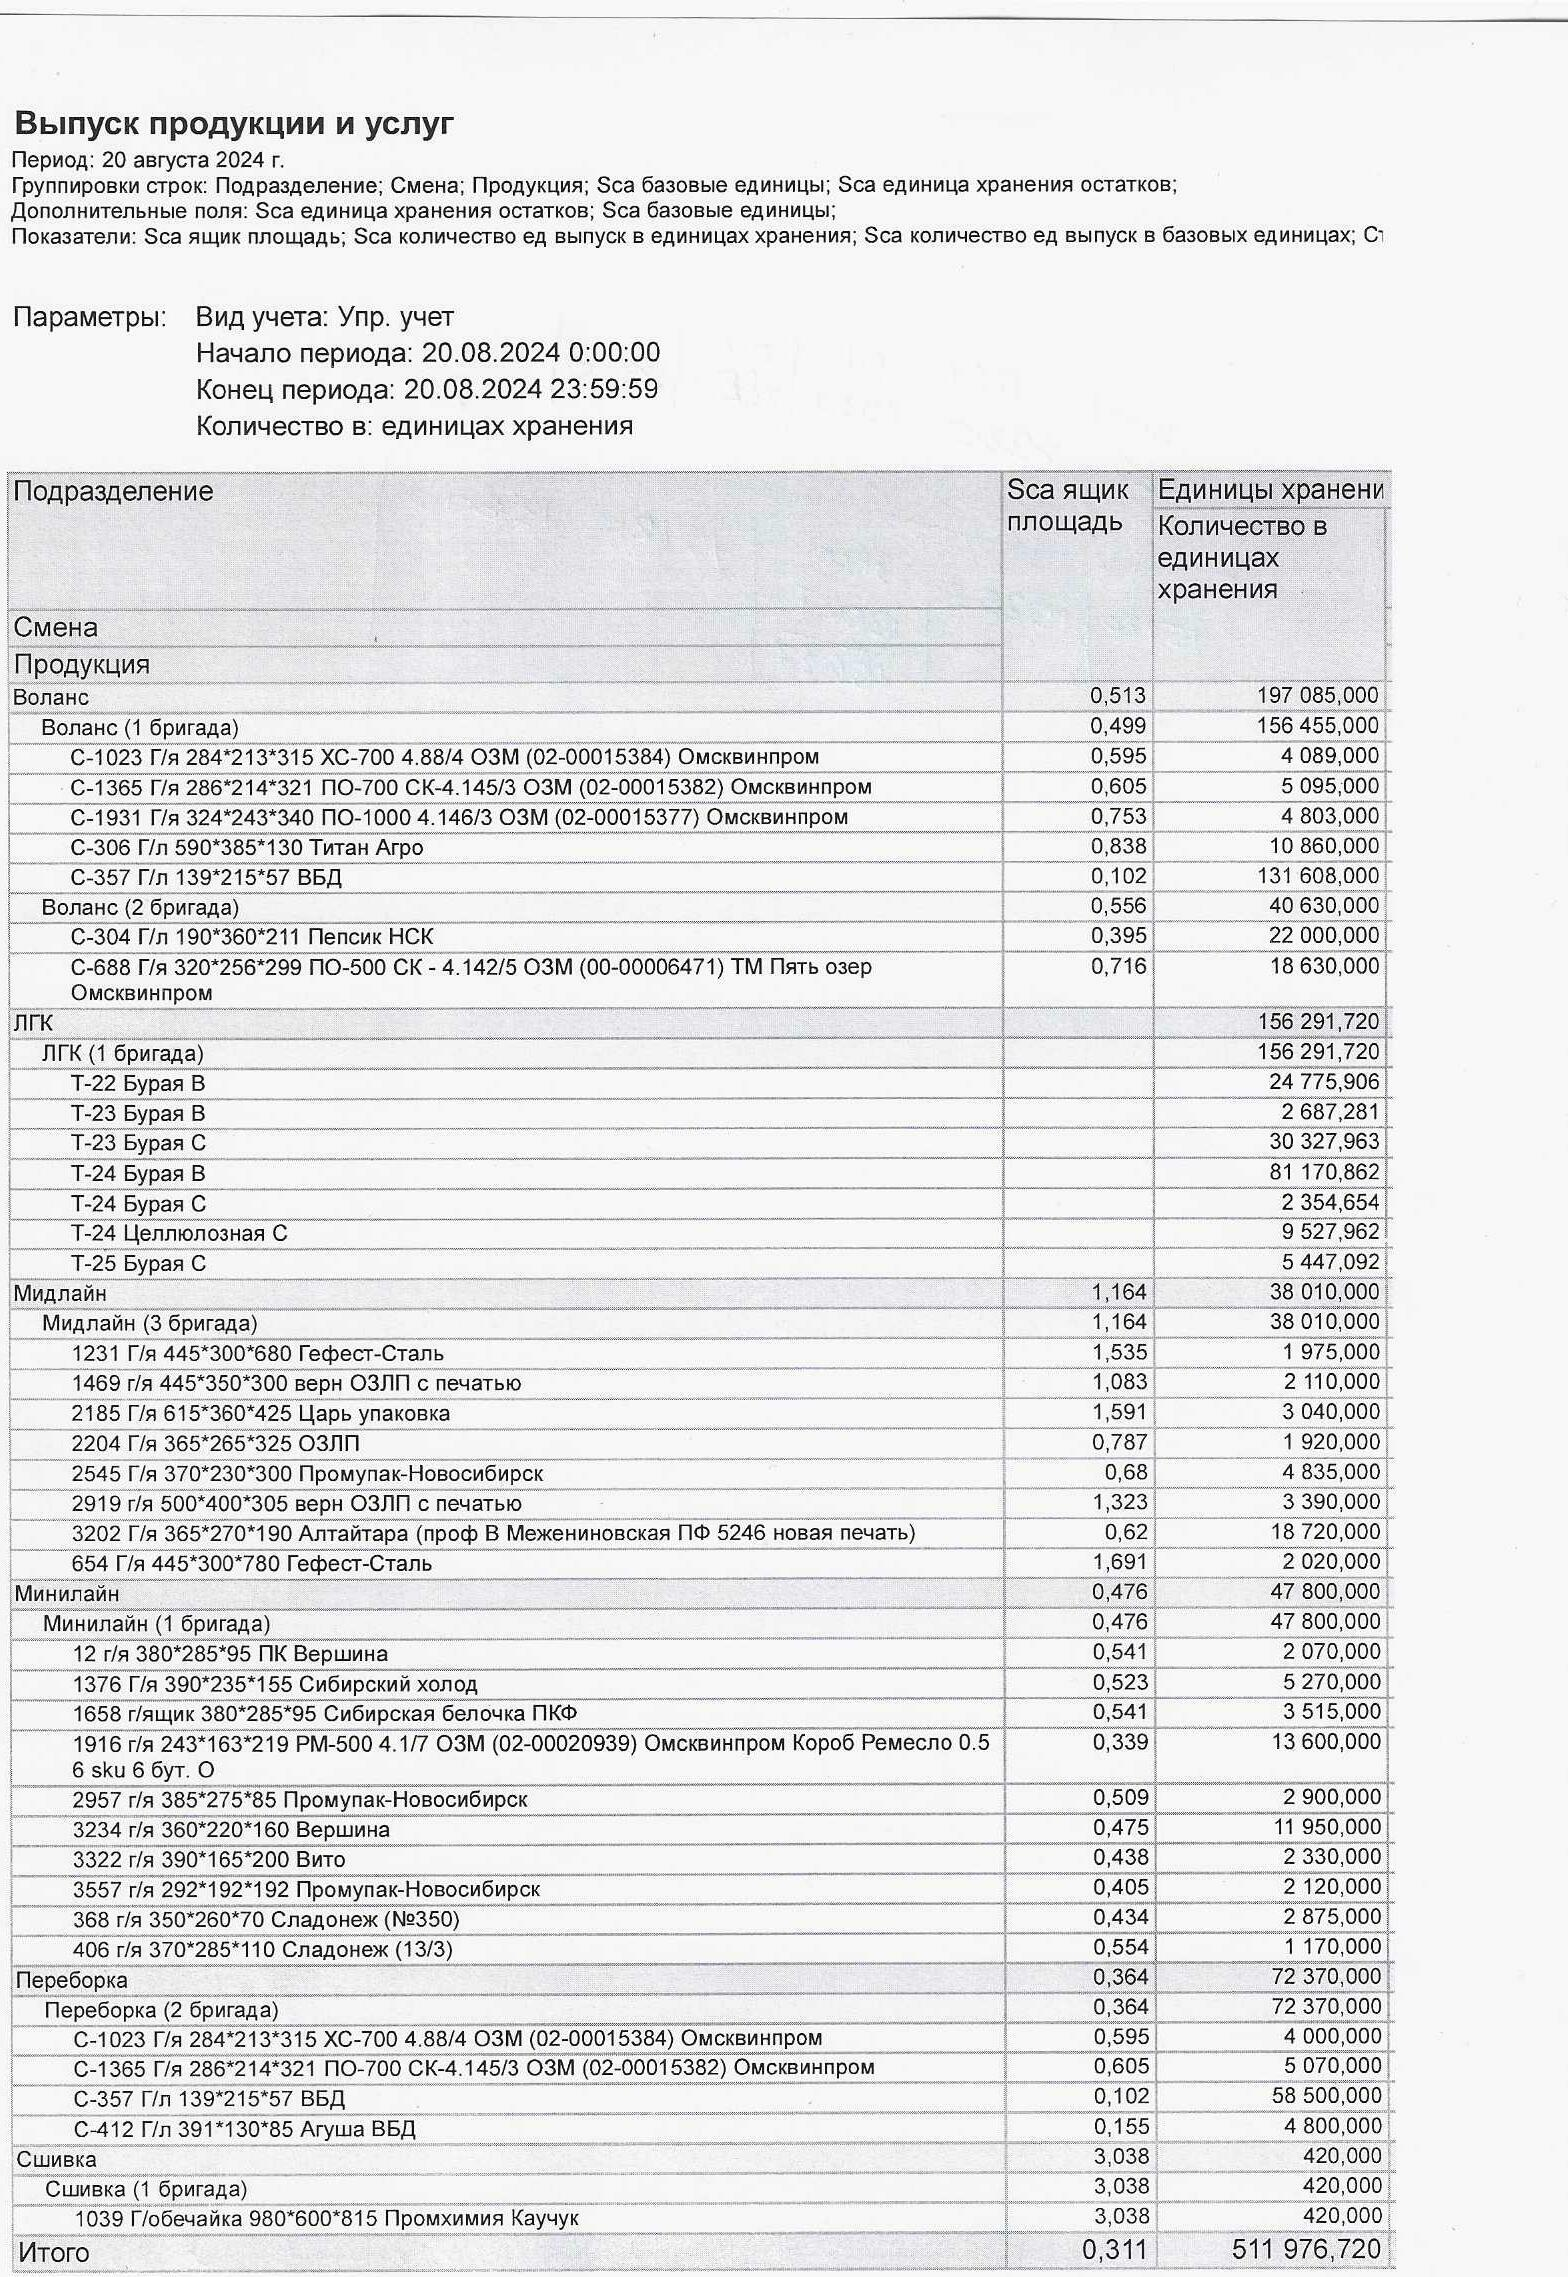
\includegraphics[height=0.94\textheight, width=0.94\textwidth, keepaspectratio]{Pics 1/0 Отчет выпуск продукции и услуг_0001.jpg}
\end{center}
  \caption{Отчет в по выпуску продукции в системе 1С:УПП}
  \label{pic:0 Отчет выпуск продукции и услуг_0001}
\end{figure}

\begin{figure}
\begin{center}
  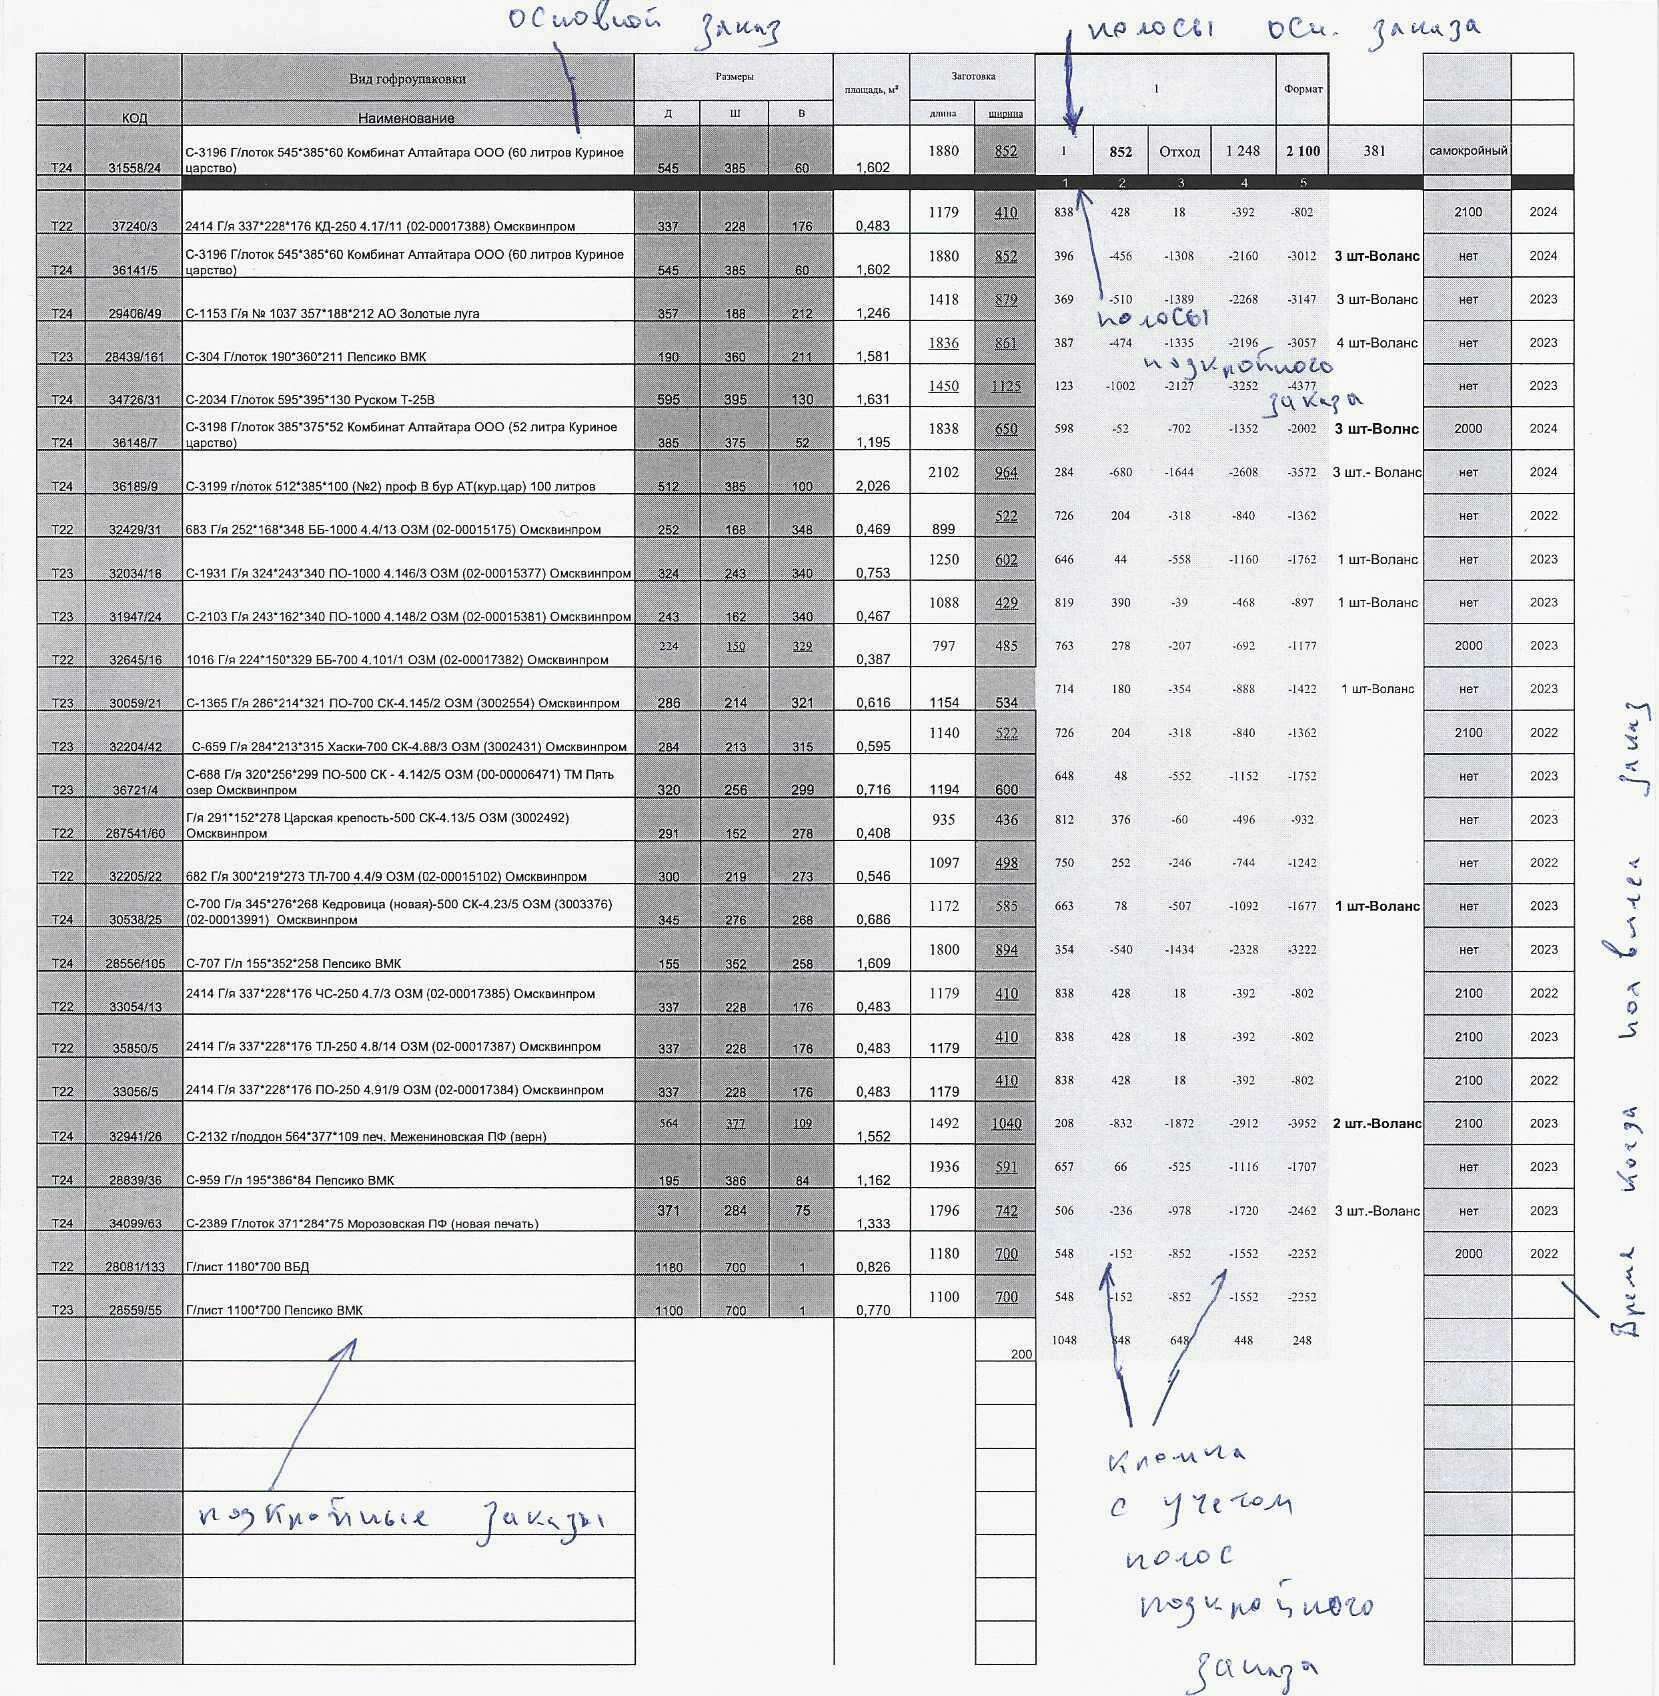
\includegraphics[height=0.94\textheight, width=0.94\textwidth, keepaspectratio]{Pics 1/0 Крой в эксель_0001.jpg}
\end{center}
  \caption{Формирование раскроев в MS Excel}
  \label{pic:0 Крой в эксель_0001}
\end{figure}

\begin{figure}
\begin{center}
  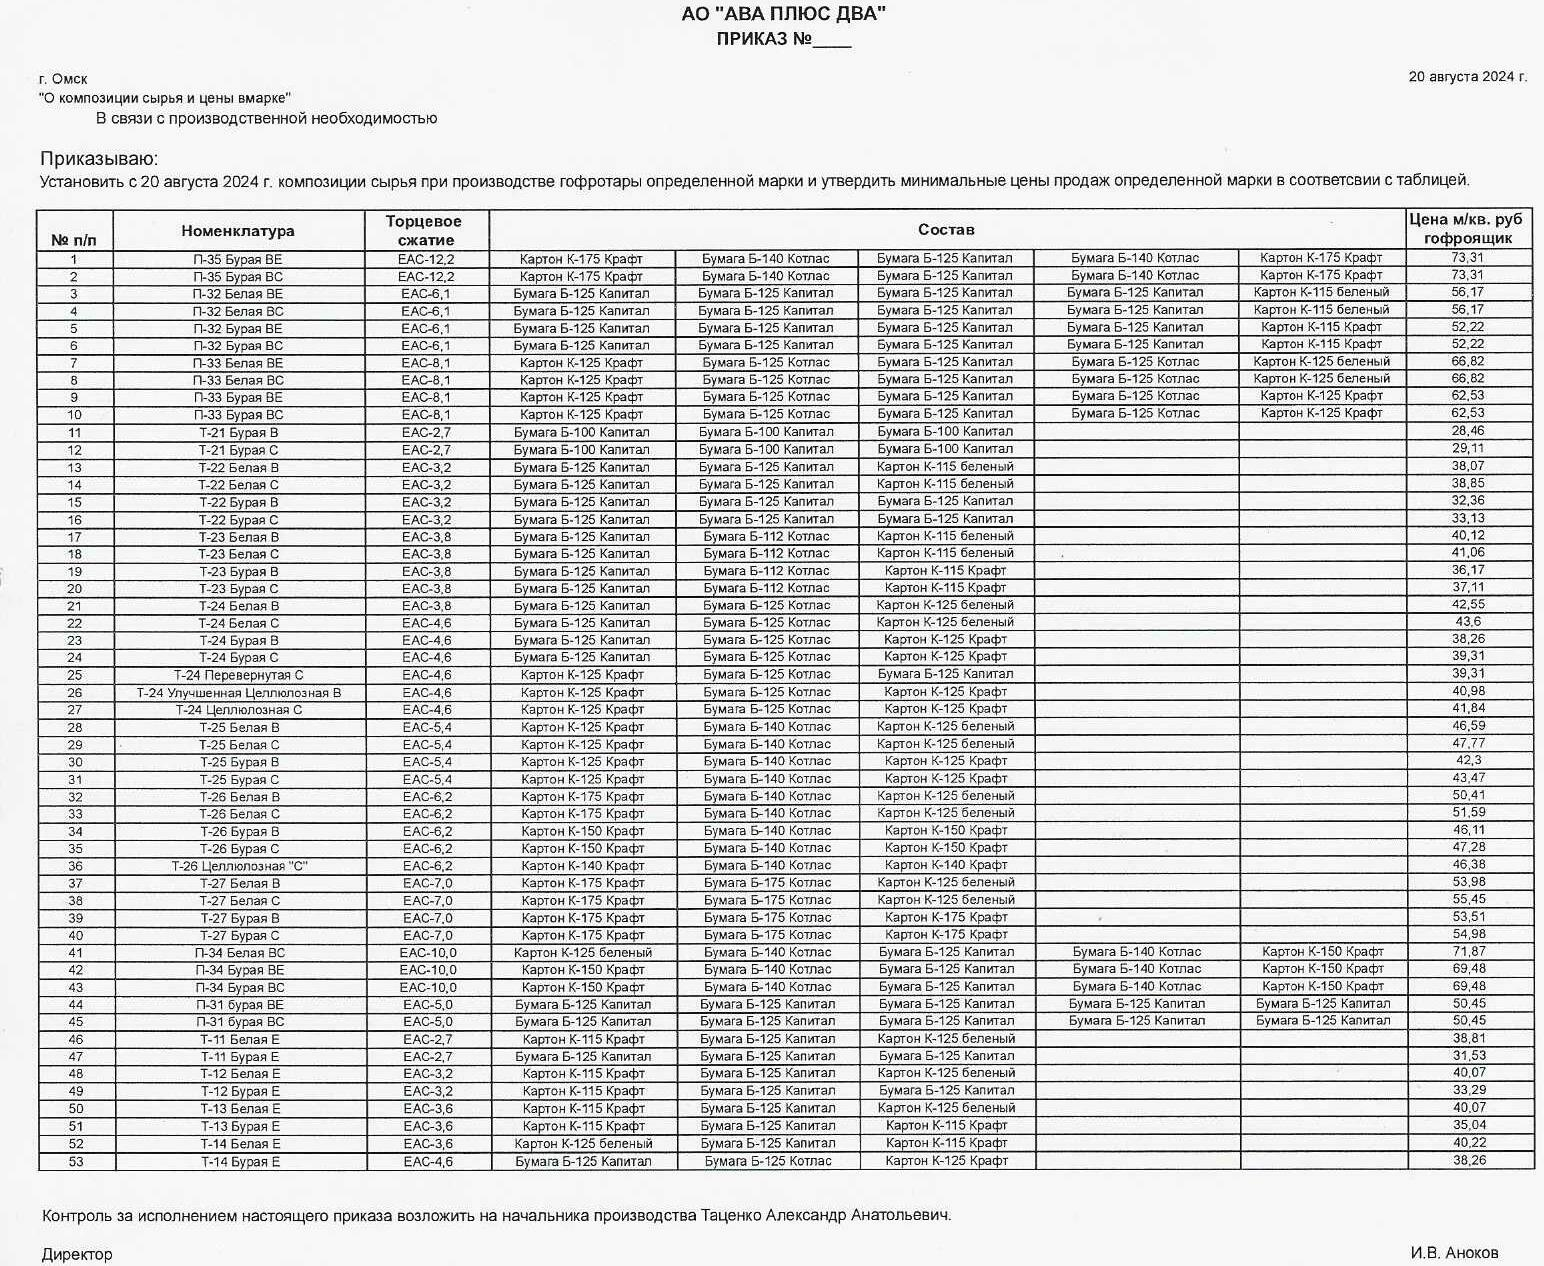
\includegraphics[height=0.94\textheight, width=0.94\textwidth, keepaspectratio]{Pics 1/0 Композиции сырья_0001.jpg}
\end{center}
  \caption{Список утвержденных композиций}
  \label{pic:0 Композиции сырья_0001}
\end{figure}

\begin{figure}
\begin{center}
  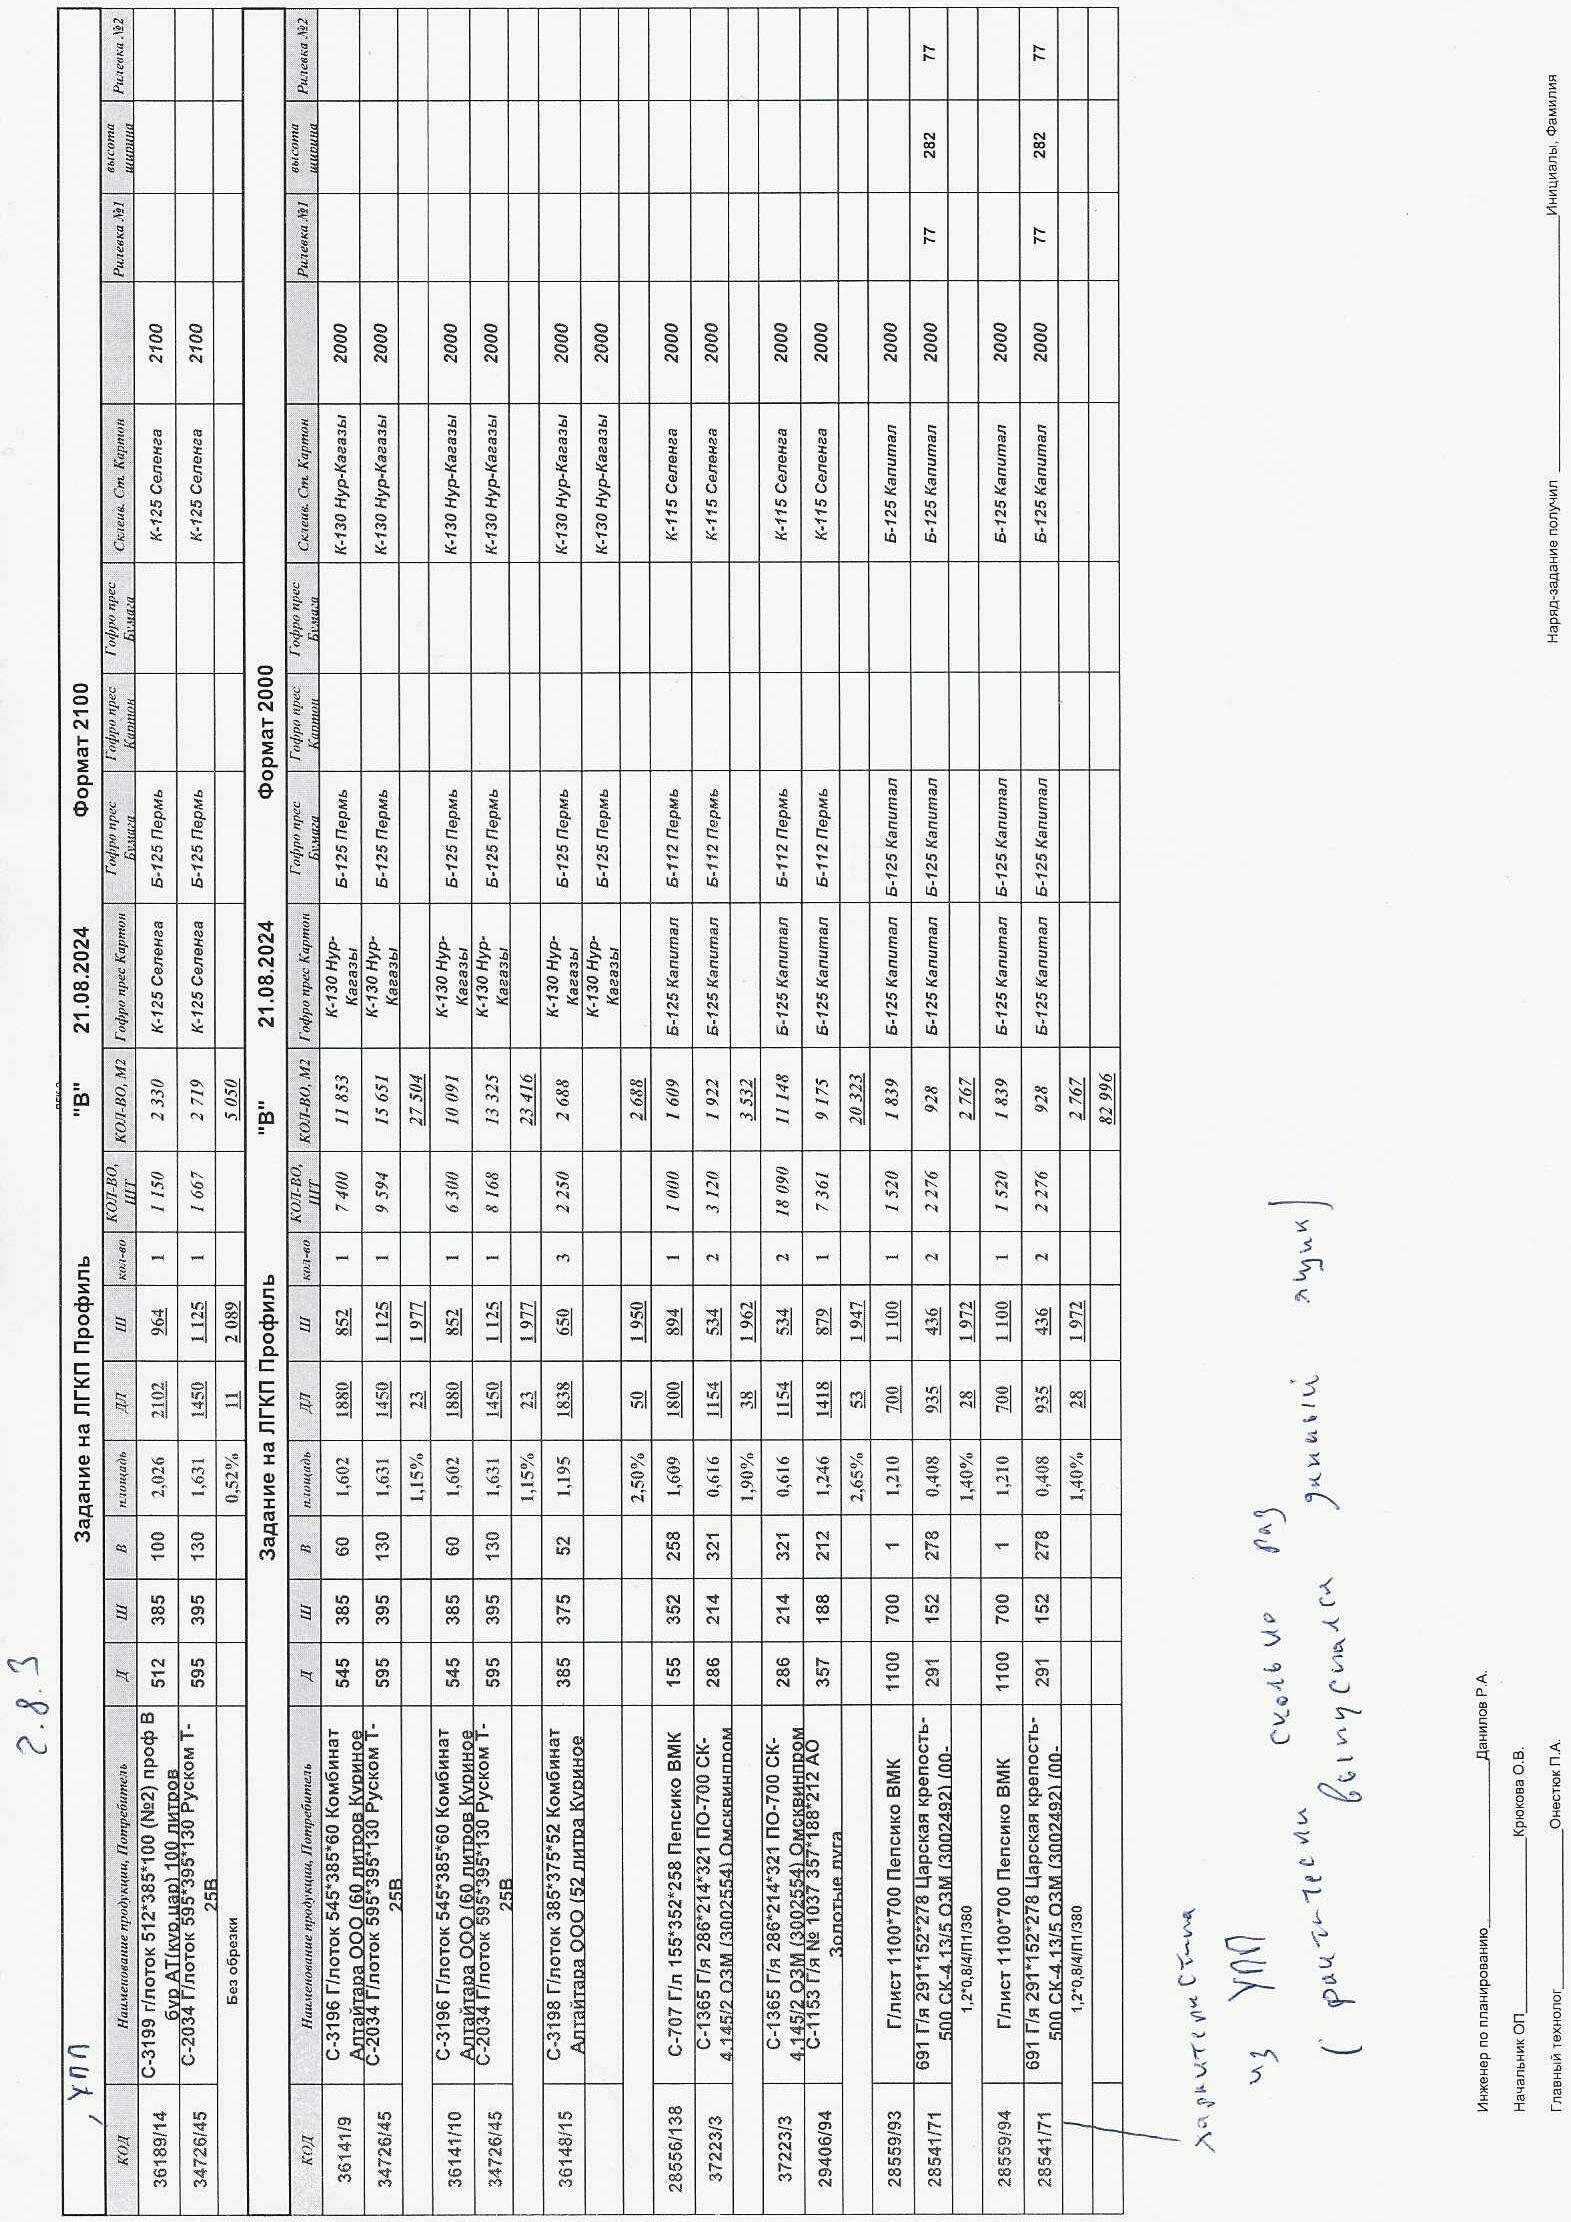
\includegraphics[height=0.94\textheight, width=0.94\textwidth, keepaspectratio]{Pics 1/2.8.3 задание от плановика на производство_0001.jpg}
\end{center}
  \caption{Задание на ГА в MS Excel}
  \label{pic:2.8.3 задание от плановика на производство_0001.jpg}
\end{figure}
%\todo{Добавить планирование в плановом отделе, планирование линий}

%Также на основании рапортов с производства планировщик ведет отчеты в таблицах MS Excel на сервере: 
%\begin{enumerate}
%     \item Отчет по %производству за период (рис. \ref{pic:pic_a23}).
%     \item Отчет по %выработке ГА и линий (рис. \ref{pic:pic_a24}).
%     \item Отчет по %простоям (рис. \ref{pic:pic_a25}).
% \end{enumerate}

%Кто-то??? распечатывает ярлыки на товарный картон (Кто?). 


% \begin{figure}
% \begin{center}
%   \includegraphics[height=0.8\textheight, width=0.94\textwidth, keepaspectratio]{Pics/Pattern.jpg}
% \end{center}
%   \caption{Заявка на приобретение продукции}
%   \label{pic:d16}
% \end{figure}
% % \clearpage



\clearpage

\ifx \notincludehead\undefined
\normalsize
\end{document}
\fi